\chapter{Opis projektnog zadatka}
		
        \section*{Uvod}

        Jedan od ključnih izazova s kojima se suočavamo u \textit{suvremenom zdravstvu} jest \textbf{neefikasnost sustava dodjele termina} i upravljanja medicinskim procesima. Područje u kojem je to zbog svoje bliskosti s "običnim" čovjekom posebno evidentno jesu \textbf{sustavi rehabilitacije}. Njih karakterizira kompleksnost potreba pacijenata, raznolikost terapijskih pristupa i ograničeni resursi, posebno izraženi u kontekstu hrvatskog zdravstva. Dosadašnji \textbf{manualni procesi} evidencije i upravljanja terminima često dovode do neoptimalnog iskorištavanja već oskudnih resursa.
        
        \subsection*{\textbf{\large Potreba za inovacijom}}
        Postoji očita potreba za razvojem \textit{novog sustava} koji će omogućiti bolje upravljanje rehabilitacijskim procesima, povećati efikasnost i znatno unaprijediti iskustvo i zadovoljstvo pacijenata.
        
        \subsection*{\textbf{\large Transformacija procesa}}
        Projekt je započeo s vizijom transformacije postojećih manualnih procesa u \textbf{automatizirani, digitalizirani sustav}. Cilj nam je bio kreiranje platforme koja optimizira raspodjelu termina, \textbf{povećava efikasnost} i pruža transparentnost u praćenju i upravljanju procesima rehabilitacije.
        
        \subsection*{\textbf{\large Inkluzivnost i dostupnost}}
        Fokus projekta bio je na razvoju \textit{inkluzivnog} servisa dostupnog za široku populaciju. Zbog toga je potrebno omogućiti jednostavno korištenje platforme za sve članove društva, uključujući pacijente i djelatnike.
        
        \subsection*{\textbf{\large Razvoj web aplikacije}}
        Ključni dio projekta uključuje razvoj web aplikacije koja bolesnicima omogućava prijavu na rehabilitaciju, odabir terapije i termine te praćenje njihovog napretka. Djelatnicima zdravstvene ustanove pruža se niz alata za efikasno upravljanje terminima i bilježenje napretka pacijenata, dok se administratorima omogućava upravljanje korisničkim računima i resursima.


        \section*{Funkcionalnost aplikacije}

        Aplikacija je zamišljena tako da omogućuje bolesnicima prijavu na rehabilitaciju i praćenje napretka te sljedećih termina u stvarnom vremenu. S druge strane, djelatnici imaju interaktivan raspored kojem mogu pristupiti u bilo kojem trenutku, dok administratori nadziru sve termine i rasporede kako bi bili sigurni da je čitav proces optimiziran. \\
        
        U našoj aplikaciji, interakcija između glavnih dionika - bolesnika, djelatnika zdravstvene ustanove i administratora sustava - ključna je za njezin uspješan rad. Svaki od ovih dionika ima specifične uloge i funkcionalne zahtjeve.
        
        \subsection*{Administratori sustava}
        \begin{itemize}
            \item \textbf{Upravljanje korisnicima:} Administratori imaju ključnu ulogu u upravljanju korisničkim računima, kako za djelatnike, tako i za bolesnike. Oni mogu prihvatiti ili odbiti registracije te uređivati ili brisati postojeće račune.
            
            \item \textbf{Nadzor termina:} Odgovorni su za pregled i potvrdu prijava bolesnika za rehabilitaciju te mogu otkazati ili pomaknuti zakazane termine.
        
            \item \textbf{Pristup i analiza podataka:} Administratori imaju pristup cjelokupnoj bazi podataka, omogućavajući im nadzor i analizu svih aspekata rehabilitacijskog procesa.
        \end{itemize}
        
        \subsection*{Djelatnici zdravstvene ustanove}
        \begin{itemize}
            \item \textbf{Bilježenje napretka:} Djelatnici mogu bilježiti napredak bolesnika tijekom rehabilitacijskih sesija, što je ključno za praćenje i prilagodbu terapijskih pristupa.
        
            \item \textbf{Upravljanje rasporedom:} Imaju mogućnost pregleda i upravljanja vlastitim rasporedom sesija, kao i pristup podacima o bolesnicima.
        
            \item \textbf{Komunikacija s bolesnicima:} Mogućnost otkazivanja sesija pod određenim uvjetima omogućava djelatnicima fleksibilnost u upravljanju izvanrednim situacijama.
        \end{itemize}
        
        \subsection*{bolesnici}
        \begin{itemize}
            \item \textbf{Proces registracije i prijave:} Bolesnici se mogu registrirati u sustav, prijaviti se i pristupiti svojim profilima za praćenje rehabilitacije.
        
            \item \textbf{Praktične mogućnosti:} Mogu se prijaviti na rehabilitaciju, odabrati terapiju, termine dolaska (koji prate pravila specifične terapije) te pratiti svoje termine i povijest terapija. U iznimnim situacijama mogu pomaknuti termin. 
        
            \item \textbf{Pristup informacijama:} Imaju pristup svom kalendaru s terminima terapije što im omogućava bolje planiranje i organizaciju.
        \end{itemize}
        
        \subsection*{Baza podataka}
        \begin{itemize}
            \item \textbf{Središnje skladište podataka:} Sve informacije o bolesnicima, djelatnicima i rehabilitacijskim sesijama pohranjuju se u bazi podataka čime se osigurava integracija i efikasnost sustava.
        \end{itemize}
        
        \eject
        
        

        \section*{Poslovni model}
        
        \subsection*{B2B model i implementacija u bolničkom sustavu}
        \begin{itemize}
            \item \textbf{Orijentacija na bolnički sustav:} Naša aplikacija je primarno namijenjena upotrebi unutar \textit{bolničkog sustava}, što je usko povezano s B2B (business-to-business) modelom. Ovaj pristup podrazumijeva da naša aplikacija nije direktno namijenjena pojedinačnim korisnicima, već bolnicama i poliklinikama kao korporativnim klijentima.
            
            \item \textbf{Razina implementacije:} Uspješna implementacija aplikacije zahtijeva široku adaptaciju, idealno na nacionalnoj razini ili barem unutar privatnih poliklinika za rehabilitaciju. Takav pristup omogućuje efikasniju koordinaciju i standardizaciju procesa rehabilitacije.
            
            \item \textbf{Značaj skalabilnosti:} Naš fokus je bio na razvoju aplikacije koja je fleksibilna i skalabilna, sposobna prilagoditi se različitim veličinama i vrstama zdravstvenih ustanova.
        \end{itemize}
        
        \subsection*{Ekspanzija i skalabilnost}
        \begin{itemize}
            \item \textbf{Faza početne implementacije:} Trenutno je aplikacija razvijena za upotrebu unutar jedne bolnice ili poliklinike za rehabilitaciju. Ovaj početni pristup omogućuje nam detaljno testiranje i optimizaciju funkcionalnosti aplikacije.
            
            \item \textbf{Strategije ekspanzije:} U razmatranju načina ekspanzije identificirali smo dva glavna pristupa:
                \begin{enumerate}
                    \item \textit{Individualizirani sustavi:} Razvijanje \textit{custom} verzije aplikacije za svaku bolnicu. Svaka ustanova imala bi svoju prilagođenu verziju aplikacije što bi moglo poslužiti kao dodatni faktor privlačnosti za klijente.
                    
                    \item \textit{Centralizirani sustav:} Stvaranje jedne velike centralizirane aplikacije. Ovaj pristup uključuje izbor institucije na početku korištenja aplikacije.
                \end{enumerate}
            
            \item \textbf{Potencijal za daljnju ekspanziju:} Oba pristupa imaju svoje prednosti i izazove te pružaju različite mogućnosti za daljnju ekspanziju i adaptaciju aplikacije, u skladu s potrebama tržišta i specifičnostima korisnika. Lako je moguće da bismo se odlučili za \textit{hibridni pristup} gdje bi svaka bolnica imala naizgled "svoju" aplikaciju "hostiranu" na \textit{custom} domeni, s vizualno prilagođenim korisničkim sučeljem (UI). Ovaj pristup kombinira prednosti individualiziranih i centraliziranih sustava omogućujući bolnicama da se osjećaju kao da imaju jedinstveno, prilagođeno rješenje dok se u stvarnosti koristi jedan centralizirani sustav.

            Pod "haubom", sve bi aplikacije bile zasnovane na istoj osnovnoj arhitekturi i dijelile isti skup funkcionalnosti. To bi omogućilo efikasnije održavanje i ažuriranje sustava dok bi korisnici imali dojam personaliziranog iskustva. Tehnički, ovakav pristup može se postići korištenjem \textit{proxy servera} ili sličnih tehnologija za usmjeravanje prometa na odgovarajuće instance aplikacije omogućujući tako svakoj bolnici da ima svoju unikatnu URL adresu i prilagođen UI. Ovaj hibridni model pruža fleksibilnost u pružanju usluga klijentima, dok istovremeno minimizira troškove i složenost održavanja više odvojenih instanci aplikacije.

            \end{itemize}
            
            \subsection*{Analiza konkurencije:} 
                Konkurenciju najbolje možemo podijeliti u dvije grupe: 
                \begin{itemize}
                    \item \textbf{Manualni sustavi:} Naša prva i najizazovnija konkurencija su postojeći manualni sustavi. Promjena navika i entuzijazam djelatnika za učenje nečega novog predstavljaju značajne prepreke.
                    \item \textbf{Digitalna rješenja:} Iako je teško pronaći konkretna B2B rješenja putem običnog pretraživanja, neka od rješenja koja smo identificirali uključuju:
                    \begin{itemize}
                        \item \textbf{MedBridge Go:} Radi se o aplikaciji koja je pretežno usmjerena odrađivanju vježbi koje je doktor propisao kod kuće. 
                        Također postoje posebni profili za liječnika i pacijenta, ali ovdje se ne delegira resursima odjela za fizikalnu terapiju te zbog toga nije direktna konkurencija. 
                        \begin{figure}[!h]
                            \centering
                            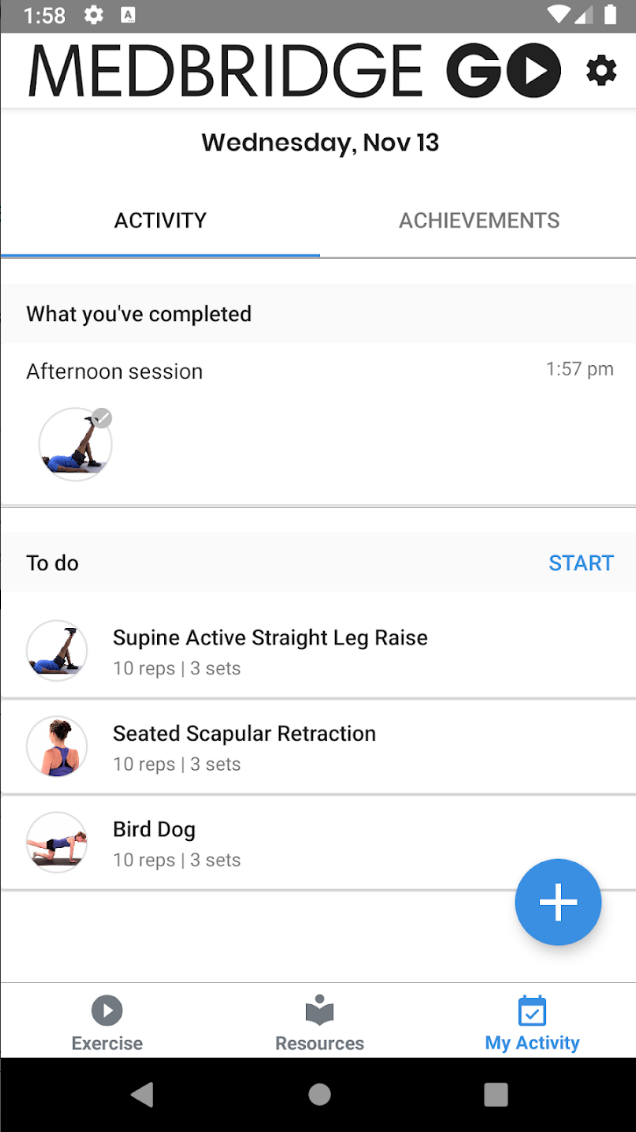
\includegraphics[width=0.35\linewidth]{slike/medbridge-go.png}
                            \caption{Sučelje aplikacije Medbridge GO koja je dostupna na pametnim telefonima}
                        \end{figure}
                        \item \textbf{BokDoc i BokDoc Partner:} Aplikacijski paket namijenjen rezervaciji termina kod doktora te promociji različitih privatnih klinika. Izgleda kao hibrid društvene mreže i oglasnika s mogućnošću narudžbe. Isto nije slična našem proizvodu. 
                        Ponovno postoje različiti profili za liječnika i pacijenta, ovoga puta to su potpuno različite aplikacije.  
                        \FloatBarrier
                        \begin{figure}
                            \centering
                            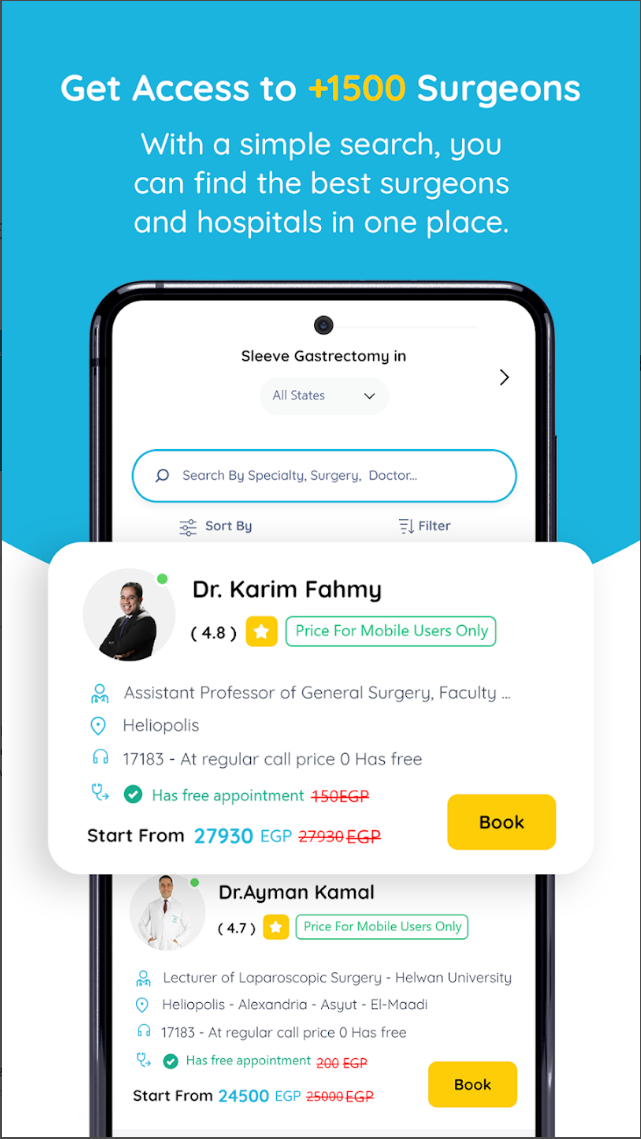
\includegraphics[width=0.35\linewidth]{slike/BokDoc.png}
                            \caption{Sučelje aplikacije BokDoc koja je dostupna na pametnim telefonima}
                        \end{figure}
                        \FloatBarrier
                        \item \textbf{Practo:} Indijska telemedicinska aplikacija koja nudi različite zdravstvene usluge. Uključuje video konzultacije, online zakazivanje, pronalazak bolnica i tretmana te čitanje zdravstvenih savjeta. Velika mreža liječnika i pružatelja zdravstvenih usluga dostupna je korisnicima. 
                        Razlikuje se od našeg proizvoda jer se fokusira na širok spektar zdravstvenih usluga, dok je naša aplikacija specifična za upravljanje procesima rehabilitacije.
                        \FloatBarrier
                        \begin{figure}[!h]
                            \centering
                            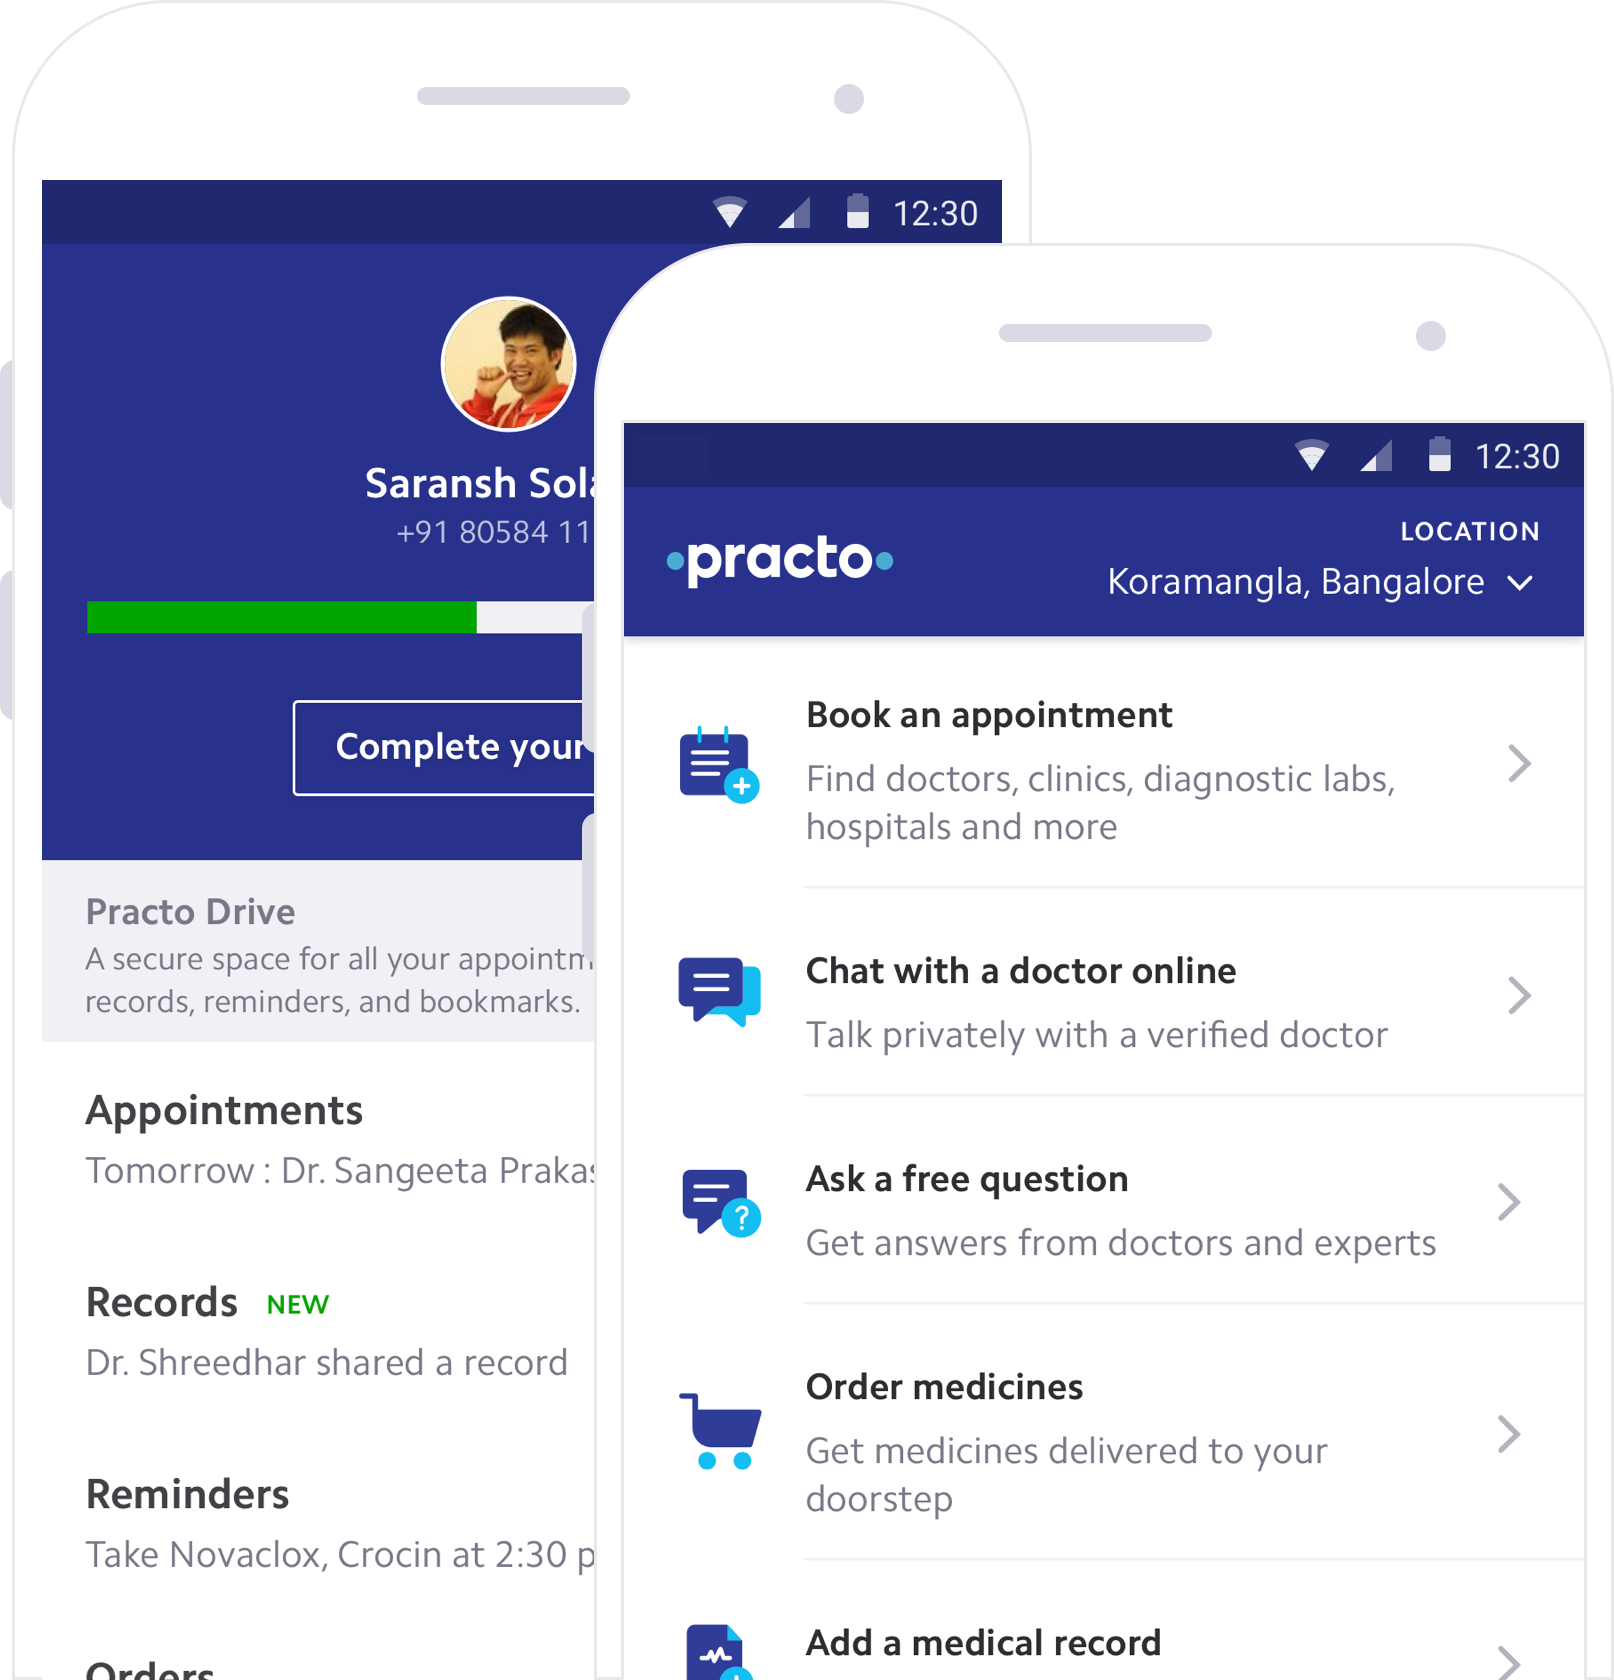
\includegraphics[width=0.5\linewidth]{slike/Practo.png}
                            \caption{Sučelje aplikacije Practo, dostupno na pametnim telefonima}
                        \end{figure}
                        \FloatBarrier
                        \item \textbf{SimplyBook.me i SimplyBook.me Admin:} SimplyBook.me je aplikacija za upravljanje terminima, posebno prilagođena korisnicima koji žele lagan pristup svojim postojećim rezervacijama. Omogućuje jednostavno dodavanje klijenata i uređivanje starih rezervacija. Korisnici primaju obavijesti o novim rezervacijama i podsjetnike za nadolazeće termine. Aplikacija je idealna za korisnike koji su često u pokretu, nemaju pristup uređajima s velikim ekranima tijekom radnog vremena ili žele provjeriti nadolazeće termine dok su kod kuće. Razlikuje se od našeg proizvoda jer je usmjerena na općenito upravljanje terminima, dok se naša aplikacija fokusira na specifične potrebe procesa rehabilitacije u zdravstvenim ustanovama.
                        \FloatBarrier
                        \begin{figure}[!h]
                            \centering
                            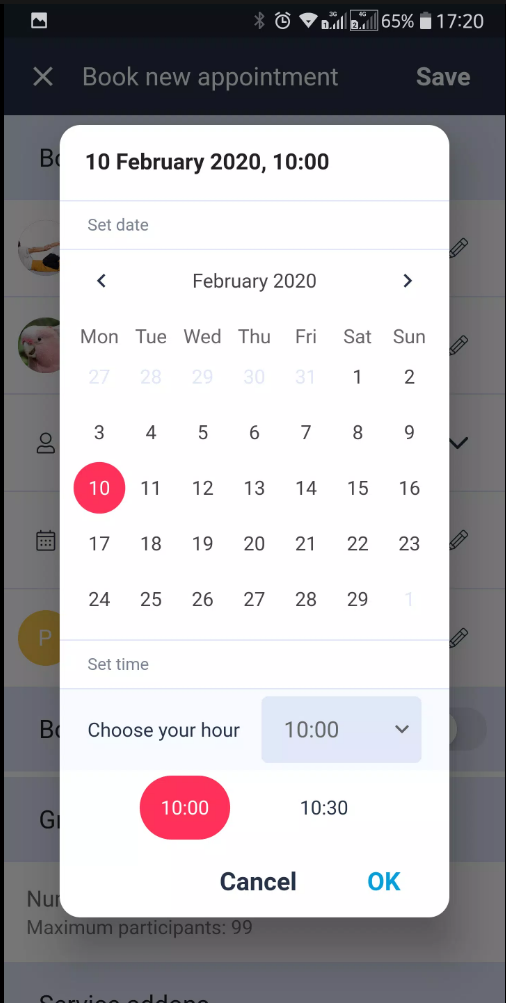
\includegraphics[width=0.45\linewidth]{slike/simplybook-client.png}
                            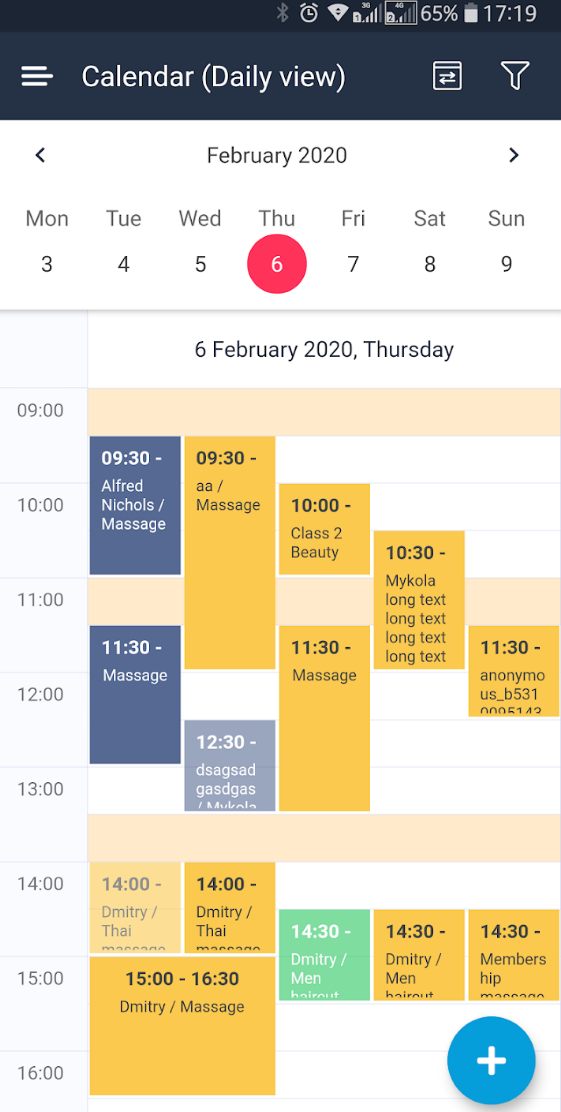
\includegraphics[width=0.45\linewidth]{slike/simplybook-admin.png}
                            \caption{Sučelje aplikacije SimplyBook.me: lijevo - korisnički pogled, desno - admin pogled}
                        \end{figure}
                        \FloatBarrier

                    \end{itemize}

                \end{itemize}


        
  
		\section*{Zaključak}

        Projekt koji smo razvili predstavlja potencijalni korak prema poboljšanju sustava rehabilitacije unutar zdravstvenog sektora. Naša aplikacija nudi inovativno rješenje koje se bavi ključnim izazovima učinkovitog upravljanja terminima i procesima, a posebno je prilagođena specifičnostima hrvatskog zdravstvenog sustava.
        
        \begin{itemize}
            \item \textbf{Inovativni pristup:} Transformacijom manualnih procesa u digitaliziranu, automatiziranu platformu aplikacija donosi povećanu efikasnost, transparentnost i bolje iskorištavanje resursa. To ne samo da unapređuje iskustvo pacijenata, već i olakšava posao djelatnicima i administratorima.
            
            \item \textbf{Fokus na korisnicima:} Razvojem aplikacije s jasnim fokusom na potrebe i udobnost korisnika posebno smo se posvetili stvaranju intuitivnog sučelja koje je pristupačno i jednostavno za korištenje svim dionicima procesa rehabilitacije.
        
            \item \textbf{Prilagodljivost i skalabilnost:} Projekt je dizajniran s obzirom na buduću ekspanziju i prilagodbu. Hibridni pristup razvoja aplikacije omogućava nam da odgovorimo na različite potrebe i zahtjeve različitih zdravstvenih ustanova nudeći im prilagođeno rješenje dok istovremeno zadržavamo unificiranu, centraliziranu strukturu.
        
            \item \textbf{Doprinos zdravstvu:} Ova aplikacija ima potencijal da značajno doprinese hrvatskom zdravstvenom sustavu koji bi osuvremenila glede procesa rehabilitacije što će imati dugoročne pozitivne učinke na kvalitetu zdravstvene skrbi.
        \end{itemize}
        
        Zaključno, ovaj projekt predstavlja važan korak naprijed u digitalizaciji zdravstvenih procesa s potencijalom da unese značajne promjene u načinu na koji se upravlja rehabilitacijom i srodnim zdravstvenim uslugama. Kroz kontinuirani razvoj i prilagodbu, ovaj sustav može služiti kao model za buduće inovacije unutar zdravstvenog sektora.
        
		
		\eject
		
	
